% Формат дипломной работы:
%     - шрифт 14
%     - бумага А4
%     - поля 2х2х2х2см
%     - полуторный межстрочный интервал
\documentclass[14pt]{extarticle}
\usepackage[paper=a4paper, top=2cm, bottom=2cm, right=1cm, left=3cm]{geometry}
\linespread{1.3}

% Стиль оглавления
%\usepackage{titletoc}
%\titlecontents{section}[2em]{\bfseries\addvspace{0.5em}}
%{\contentslabel[\thecontentslabel]{1.7em}}
%{}{\titlerule*[1pc]{.}\contentspage}

\usepackage[utf8]{inputenc}                % Кодировка
\usepackage[british]{babel}  % Русский язык
\usepackage[pdftex]{graphicx}              % Картинки

\setlength{\parindent}{0pt}
\setlength{\parskip}{1em}

\begin{document}
    \thispagestyle{empty}
\begin{center}
    \ \vspace{-3cm}

    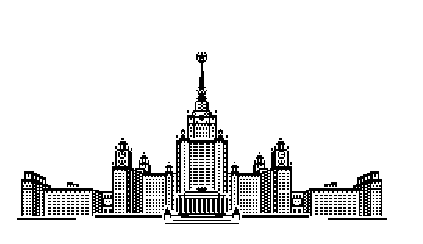
\includegraphics[width=0.5\textwidth]{title_page/msu.eps}\\

    {\small{\scshape  Lomonosov Moscow State University}\\
    Faculty of Computational Mathematics and Cybernetics\\
    Department of Systems Analysis}

    \vfill

    {\Large Kirill Egorov}

    \vspace{1cm}

    {\LARGE\bfseries Optimal Control Problem\par and methods for its solution}

    \vspace{1.5cm}

    {\scshape Abstract}
\end{center}

\vspace{3cm}

\begin{flushright}
    \large
    \textit{English lecturer}\\
    Irina Gudilina 
\end{flushright}

\vfill

\begin{center}
    Moscow, 2022
\end{center}

\clearpage
    \tableofcontents
    \clearpage
    \section{Introduction}
    The shortest path problem, or stagecoach problem, is one of the problems in graph theory with the aim of finding the optimal route between two points that minimizes the distance traveled (or the cost of the trip).

    Shortest path algorithms are used to automatically find routes between physical locations, such as driving directions on map websites such as Google Maps. When constructing a route, the vertices of the graph are road intersections, and the edges are the roads connecting them. Each edge is weighted by the time it takes a car to travel that section of road, given current traffic data.

    In networking or telecommunications thinking, this shortest path problem is sometimes called the minimum delay path problem. For example, the algorithm can search for a path on the Internet between a client and a server with the fastest path, or with the widest transmission channel.

    A more lighthearted application is a way to solve a Rubik's Cube using shortest path algorithms. Thus, if the vertices represent the states of this puzzle, and each directed edge corresponds to one move or turn, shortest path algorithms can be used to find a solution that uses the fewest possible moves.

    Other applications often studied in operations research include plant and facility layout, robotics, transportation, and others.

    This work is devoted to classical algorithms for solving the shortest path problem, which use a deterministic approach.
    These algorithms are basic and widely known. They are first in line for adoption, although large corporations have taken a different approach in recent years.
    It is customary for them to invent, for each individual problem of the optimal path, based on internal data heuristics, to build quasi-shortest paths, significantly reducing the running time of the algorithms.
    Indeed, as will be seen from this paper, the asymptotic behavior of classical algorithms leaves much to be desired.
    In fact, the new algorithms of recent years are improvements to the basic ones using additional assumptions about the nature of the data from which the graph is built.
    Therefore, it seems important to give a review of the main algorithms.

    The paper gives brief characteristics and the main idea of each of the algorithms.
    The best situation for application is described and an estimate of the algorithmic complexity for each of the algorithms is given (if it is possible to talk about algorithmic complexity in the context of a particular algorithm).

    
    \section{Formulation of the problem}
    Consider a directed graph with N nodes (vertices) and M edges.
    We will regard sequential movement from one vertex to another along the edges.
    An edge connects some two vertices to each other, movement along the edge is possible only in one direction.
    To each edge we will associate a certain number, which we will call the cost (or length).
    For a complex path passing through several vertices, the length is defined as the sum of the lengths of the edges along which the movement took place.
    A path is called the shortest path if it has the shortest length among all paths starting and ending at the given vertices.
    The shortest path problem is to find the shortest path between these two vertices.

    The shortest path problem can also be formulated differently.
    If we go back to the original definition and define the cost precisely as the cost, and not the length, then the problem in its essence can be reduced to the cheapest possible transfer of one flow unit between a pair of vertices.
    Such problems are widely studied in economic theory when considering the movement and distribution of material goods.
    This allows us to formulate the problem of finding the shortest path by defining a linear function similar to the function that defines the minimum cost flow problem.

    Thus, the formulation of the problem turns out to be broader than just finding a road on the surface of the earth, and contains space for interpretations and applications. This determines a large number of scientific fields in which these algorithms are applied.

    
    \subsection{Formulation kinds}
    There are a number of main variants of the shortest path problem. Next, we will group the algorithms according to the type of formulation they deal with. Depending on the formulation of the problem, the algorithms change their basic characteristics, such as performance, the data structures used, and the main idea.

    \textit{Finding the shortest path between a pair of vertices.}
    For a given pair of vertices, it is necessary to find the shortest path between them.
    It is worth noting that there is still no known algorithm that solves this problem asymptotically in the worst case better than the best algorithm for the problem with one initial vertex.

    \textit{Finding shortest paths with one initial vertex.}
    For a given vertex, it is necessary to find the shortest path to each of all the vertices of the graph.

    \textit{Finding shortest paths with one vertex.}
    This is the reverse side of the previous option --- you need to find the shortest path from each of the vertices of the graph to a given vertex.
    By flipping each of the edges of the graph, we get the previous problem.

    \textit{Finding shortest paths between all pairs of vertices.}
    It is necessary to find the shortest path between each pair of graph vertices.
    The solution to this problem can be obtained by solving the shortest path problem with one starting vertex for each of the vertices in the graph.

    
    \subsection{Problem assumptions}
    When solving the problem of the shortest path, we will use some assumptions.
    Assumptions are needed not so much to limit the list of algorithms, but to highlight the differences between algorithms through the prism of the relationship to these assumptions.
    Some algorithms, for example, can go in cycles when the assumption is not met, while others, on the contrary, speed up the work.
    The answer to the question which of the above assumptions satisfies the task is determined by the initial design of the system and the choice of the algorithm used.
    
    \textit{The considered graph is directed.}
    It is worth remembering that any undirected graph can be easily represented in a directed form.
    A number of algorithms also require that the edge weights be non-negative, in which case the following assumption is not necessary.
    
    \textit{The graph under consideration does not contain negative cycles.}
    A negative cycle is a path from some vertex to itself with a negative length.
    This situation is sometimes encountered in trading on the stock exchange and is studied in financial mathematics.
    From the point of view of our problem, the presence of negative cycles does not allow us to implement the algorithm in polynomial time.
    This means that such algorithms cannot be applied even on computers.

    \textit{There is at least one path between two vertices, between which we are looking for the shortest path.}
    Indeed, it seems impossible to find the shortest path in a graph if there is no connection at all between the given vertices.
    At the same time, one part of the algorithms reports that nothing was found as a result of the search, while the other part goes into an infinite loop and requires a manual stop.

    \textit{All further considerations are given for edge lengths that are integers.}
    It seems reasonable to describe algorithms for computers.
    Real and even more so complex lengths seem here to be too complicated a solution from the point of view of computer processing speed and ease of representation.

    The solution of the shortest path problem finds its application in a number of areas, such as transport or routing in communication networks and is often associated with finding a tree of shortest paths in a graph.
    
    It can be proved that the shortest paths from one node of the graph to all other nodes form a tree of shortest paths.
    This tree is interesting in that its root is formed from a given vertex, and all its edges are directed in the direction opposite to the vertex, and every path that can be laid from the original vertex to any other vertex is the shortest.
    
    \section{Solving Algorithms}
    Shortest path algorithms have many common properties.
    They are all iterative and assign each node some minimum distance from the original vertex.
    The algorithms also support a certain set of valid (sometimes unvisited) vertices.
    Although each individual implementation allows different data structures to be used to implement and represent these basic interactions, the main differences lie in the way the distance labels are updated and the selection of a candidate vertex to exit from the supported allowed set.
    According to this criterion, we will divide the algorithms into two groups:

    \textit{The label is set once.}
    These algorithms set a permanent price label for one of the tops at each step.
    This is equivalent to removing the given vertex from the available set.
    The main algorithmic complexity is mainly represented by the choice of a vertex that should leave this set.
    These algorithms are in principle inapplicable to graphs containing cycles, unless a constraint on the non-negativity of each of the lengths is required.

    \textit{The label changes while the program is running.}
    Such algorithms make it possible to correct labels on vertices by alternately deleting and adding back to the admissible set.
    The ability to change labels makes the process of choosing the next vertex less algorithmically expensive.
    Such algorithms can be used for all types of problems.
    
    It is clear that the algorithm with a one-time creation of labels is a special case of an algorithm that allows changing labels.
    Thus, the second type allows solving a larger class of problem statements.
    From a practical point of view, this flexibility has a great influence on the preferential choice of the second type by the algorithm for solving a particular problem.
    
    Another reason for choosing one or another type of algorithm is the ratio of the number of edges to the number of vertices in the graph under consideration.
    The search algorithm for the next available vertex for the first type of algorithms has linear complexity with respect to the number of nodes.
    At the same time, repeated traversal of nodes to correct labels has a linear complexity with respect to the number of edges.
    Thus, it is better to solve the problem for dense graphs by the first type of algorithms, and for sparse graphs --- by the second.
    Of course, this remark applies only to graphs without negative cycles.


    \subsection{Algorithms ``One To All''}
    Here I will describe algorithms for finding the shortest path from a given vertex to all other vertices of the graph in question.
    As noted above, the vertex-to-vertex problem, which is a special case of this one, does not currently have a solution with a better algorithmic complexity.
    Features of the construction of each algorithm affect the difference in performance under different initial conditions.
    
    \textit{Dijkstra's algorithm.}
    Dijkstra's algorithm is one of the most famous and productive algorithms known today.
    It belongs to the first type of algorithms, that is, each node is labeled only once.
    Initially, the set of visited vertices consists of one given source vertex with distance zero.
    Then, at each iteration, the element with the smallest length is selected from this set.
    For each neighbor, a label is placed with a length equal to the sum of the distance to the selected vertex and the length of the edge.
    Neighbors are removed from the set of visited vertices.
    Thus, at each iteration of the algorithm, it is necessary to search for a minimum over the set of visited vertices, which is generally done in linear time.
    Thus, the final complexity of the algorithm is quadratic with respect to the number of nodes in the considered graph.

    Dijkstra's algorithm has proven itself to be the most reliable and understandably modifiable (in the sense that specific points for potential improvements are clear).
    At the same time, even the basic version has a pretty good performance.
    Therefore, most of the algorithms from the list are a superstructure on Dijkstra.
    Further, I will not redefine the basic structures, as the set of visited vertices, for such algorithms, but only mention their specific implementations and the resulting performance gains.

    \textit{Dijkstra's Heap Algorithm.}
    This algorithm differs from the previous one by using a special data structure to represent the set of visited vertices.
    If you use a priority queue (also called a heap) instead of a standard list, you can achieve a significant increase in the speed of searching for the maximum.
    The priority queue maintains a minimum at the top of the heap, and it takes logarithmic time to rebuild it.
    Then the complexity will be linear in the number of edges and linear-logarithmic in the number of nodes.
    
    \textit{Dial's algorithm.}
    These are improvements to Dijkstra's algorithm for detecting when the weights are integer, positive, and there are few variations of different lengths relative to the number of vertices.
    Then it is customary to use an array of buckets to store a set of unvisited vertices, each of which will store vertices with the same label.
    To find the minimum, then it is enough to find the first non-empty bucket from the list.
    In some cases, this can reduce the complexity of the entire algorithm to a linear one.
    Also, this algorithm can be used to search for quasi-shortest paths, if the first item in the functional requirements for the system is its performance.

    \textit{Bellman--Ford algorithm.}
    Based on the principles of dynamic programming, this algorithm is the only one of the second type in this list.
    Its idea is to sequentially recalculate labels for all graph nodes without exception until the optimal path value is found.
    It is proved that it is enough to make as many iterations as there are nodes in the graph to stop.
    This algorithm allows you to set negative distances, cycles, and also indicates the presence of a negative cycle, if it is present in the graph.
    Stops from using this algorithm its large quadratic algorithmic complexity.

    In this case, the algorithm is based on principles that are applied in areas of mathematics other than discrete, in particular, optimal control.
    Moreover, there are similar results for continuous cases.
    This allows us to consider the Bellman--Ford algorithm as an independent subject of study, and attempts to use it to connect the continuous world with a discrete mathematical model inside a computer.

    \textit{Using quasi-sorted lists to store a list of unvisited vertices.}
    If each of the vertices considered at this iteration is added to the beginning or end (middle) of the list of unvisited vertices, depending on some condition, then it is possible to predictably reduce the search time for the minimum in this data structure.
    In this case, the resulting minimum will not be strict, that is, the probability that the vertex selected at the current iteration will be added back to the list at one of the next iterations will remain.
    Usually, strategies are used less than the first at the beginning, more than the last at the end, and various combinations of them.
    It is not possible to give an exact estimate of the complexity of these algorithms, because it depends on each specific graph.
    Perhaps there are probabilistic estimates for special cases of such an algorithm.

    Note that there are a number of articles claiming that this type of algorithm is the fastest for the problems they considered.
    These problems are of a rather general nature, which adds credibility to their conclusions. At the same time, of course, it is impossible to call the existence of these articles a proof in the strict mathematical sense.

    
    \subsection{Algorithms ``All To All''}
    In this section, I present the basic algorithms for solving the problem when it is necessary to build the shortest paths from each point of a given graph to each of the remaining ones.

    Due to the fact that these algorithms are rarely used because of performance problems, it is not possible to reliably describe the most common implementation of the data structures used by the algorithm. I will describe only the basic principle of constructing these algorithms and the minimum possible algorithmic complexity for this principle.

    \textit{Doubling algorithm.}
    The idea of the algorithm is to sequentially enumerate all paths for a fixed target node.
    First, the shortest path is chosen from all paths of length 1, then of length 2, and so on.
    This iterative process is similar to the process of matrix multiplication.
    Indeed, the adjacency matrix can be used to create a matrix of a special type, the multiplication of which by itself will give the result of the program at the next iteration.
    Such an algorithm has the fourth degree of algorithmic complexity.
    A possible improvement is to multiply only the largest powers of the matrices improve the overall asymptotics, but only up to the cube per logarithm of the total number of vertices in the graph.
    
    \textit{Floyd--Warshall algorithm.}
    The idea of the algorithm is to fix at each iteration a number from one to the total number of vertices.
    During iteration, the minimum distances for all nodes of the graph are calculated with the constraint that all paths must necessarily pass through the first nodes, limited by the chosen number.
    The implementation of such an algorithm is quite naive (consists of three nested loops) and has cubic complexity.
    
    \textit{Johnson algorithm.}
    The algorithm runs Dijkstra's algorithm discussed above for each of the vertices of the graph.
    Usually, before using the main process on the graph, the Bellman--Ford algorithm is run with a fictitious starting vertex to determine the presence of negative edges that Dijkstra's algorithm cannot work with.
    In the case of found negative edges, it is required to replace the lengths of edges in accordance with the lemma on changing the lengths of edges in a weighted graph, and such a replacement is carried out for each edge separately using the shortest weights from a fictitious vertex previously calculated by the Bellman--Ford algorithm.
    Johnson's algorithm is the most productive algorithm today.
    Its complexity can be computed as linear times the complexity of Dijkstra's algorithm (depending on the specific implementation).
    
    
    \section{Conclusion}
    The paper presents the basic solutions of the shortest path problem for various formulations of this problem.
    The above algorithms can be used as a basis for writing heuristic quasi-shortest path algorithms, or for direct application while meeting the functional performance requirements of the algorithms.

    The main ideas of the algorithms and their performance characteristics (operational complexity of the algorithm depending on the number of nodes or the number of edges) are described.
    
    Based on the above information, a picture of the frequency of application of algorithms is formed.
    ``All-to-all'' algorithms have monstrously poor performance.
    Therefore, they are not used even for tasks where the response time to the user is the most important functional requirement.
    Indeed, how long can it take to calculate the travel time between all road intersections in Moscow?
    The Bellman--Ford algorithm is only of interest to the scientific public, as an alternative to Dijkstra and behind which stands the whole mathematical theory of Bellman's dynamic programming.
    Some may see space here for scientific discovery.
    Basically, they use various variations of Dijkstra's algorithm, which are built for the data used, give the expected priority directions, and apply other tricks to increase performance.

    The paper presents the main assumptions that must be remembered when applying these algorithms and describes the relationship of each of the algorithms to the corresponding assumptions.
    The cases of the most favorable use of algorithms as a result of listing the advantages and disadvantages of these algorithms are also given.

    This work will be useful for novice programmers who solve problems on graphs, as it introduces readers to the basic algorithms and principles of their classification, which are universal for this area of mathematics.
    
    \begin{thebibliography}{9}
        \bibitem{} Ahuja, Ravindra K.; Mehlhorn, Kurt; Orlin, James; Tarjan, Robert E. (April 1990). ``Faster algorithms for the shortest path problem''. Journal of the ACM. ACM. 37 (2): 213–223.
        \bibitem{} Bellman, Richard (1958). ``On a routing problem''. Quarterly of Applied Mathematics. 16: 87–90.
        \bibitem{} Dantzig, G. B. (January 1960). ``On the Shortest Route through a Network''. Management Science. 6 (2): 187–190.
        \bibitem{} Fredman, Michael Lawrence; Tarjan, Robert E. (1987). ``Fibonacci heaps and their uses in improved network optimization algorithms''. Journal of the Association for Computing Machinery. 34 (3): 596–615.
        \bibitem{} Pettie, Seth (26 January 2004). ``A new approach to all-pairs shortest paths on real-weighted graphs''. Theoretical Computer Science. 312 (1): 47–74.
    \end{thebibliography}
\end{document}


